\section*{Endliche Automaten}

\begin{definition}{Endliche Automaten}
    Maschinen, die Entscheidungsprobleme lösen\\
    \begin{minipage}{0.35\linewidth}
        \begin{itemize}
            \item Links nach rechts
            \item Keinen Speicher
            \item Keine Variablen
        \end{itemize}
    \end{minipage}
    \begin{minipage}{0.5\linewidth}
        \begin{itemize}
            \item Speichert aktuellen Zustand
            \item Ausgabe über akzeptierende\\ Zustände
        \end{itemize}
    \end{minipage}
\end{definition}

\begin{definition}{DEA} deterministischer endlicher Automat: $M=(Q, \Sigma, \delta, q_{0}, F)$

    \begin{minipage}{0.5\linewidth}
        $Q$: endliche Menge von Zuständen

        $\Sigma$: endliches Eingabealphabet

        $\delta: Q \times \Sigma \rightarrow Q$ Übergangsfunktion
    \end{minipage}
    \hspace{1mm}
    \begin{minipage}{0.4\linewidth}
        $q_{0} \in Q$ Startzustand

        $F \subseteq Q$ Menge der\\ akzeptierenden Zustände
    \end{minipage}
\end{definition}

\begin{KR}{DEA Funktionen}
    $M=\left(Q, \Sigma, \delta, q_{0}, F\right)$ : EA\\ 
    Konfiguration $M$ auf $\omega$ $\in$ $Q \times \Sigma^{*}$
    (Start: $(q_{0}, \omega)$, End: $(q_{n}, \varepsilon)$)
    
    Berechnungsschritt $\vdash_{M}$ von $M$:
    $
    (q, \omega) \vdash_{M}(p, x)
    $

    Berechnung: \\{\small $(q_{a}, \omega_{1} ... \omega_{n}) \vdash_{M} ... \vdash_{M}(q_{e}, \omega_{j} ... \omega_{n}) \rightarrow(q_{a}, \omega_{1} ... \omega_{n}) \vdash_{M}^{*}(q_{e}, \omega_{j} ... \omega_{n})$}
   
\end{KR}

\begin{example2}{Beispiel DEA (eindeutig)} Sprache: $L(M)=\left\{1 x 1 \mid x \in\{0\}^{*}\right\}$
    
    \begin{minipage}{0.45\linewidth}
        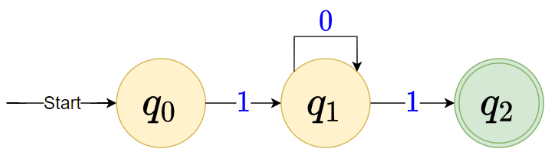
\includegraphics[width=1\linewidth]{images/dea_example.png}
    \end{minipage}
    \hspace{1mm}
    \begin{minipage}{0.5\linewidth}
        \textbf{Konfiguration} auf $\omega=101$
        \begin{itemize}
        \item Startkonfiguration $\rightarrow\left(q_{0}, 101\right)$
        \item Endkonfiguration $\rightarrow\left(q_{2}, \varepsilon\right)$
        \end{itemize}
    \end{minipage}

    \textbf{Berechnung}

    \resizebox{\linewidth}{!}{
    $\omega=101 \rightarrow\left(q_{0}, 101\right) \vdash_{M}\left(q_{1}, 01\right) \vdash_{M}\left(q_{1}, 1\right) \vdash_{M}\left(q_{2}, \varepsilon\right) \rightarrow \text{akzeptierend}$\\
    }

    
    $\omega=10 \rightarrow\left(q_{0}, 10\right) \vdash_{M}\left(q_{1}, 0\right) \vdash_{M}\left(q_{1}, \varepsilon\right) \rightarrow \text{verwerfend}$
    
\end{example2}


\begin{definition}{Nichtdeterministischer endlicher Automat (NEA)}
    
        Unterschied zum DEA: Übergangsfunktion $\delta: Q \times \Sigma \rightarrow P(Q)$\\
        Ein $\varepsilon$-NEA erlaubt zusätzlich noch $\varepsilon$-Übergänge
\end{definition}




\begin{formula}{Teilmengenkonstruktion}
    $\forall$ NEA kann in DEA umgewandelt werden
    \begin{enumerate}
        \item $Q_{N E A} \rightarrow P\left(Q_{N E A}\right)=Q_{D E A} \quad$ (Potenzmenge)
        \item Verbinden mit Vereinigung aller möglichen Zielzustände
        \item Nicht erreichbare Zustände eliminieren
        \item Enthält akzeptierenden Zustand $=F_{N E A} \rightarrow$ akzeptierend
    \end{enumerate}

    \begin{minipage}{0.5\linewidth}
        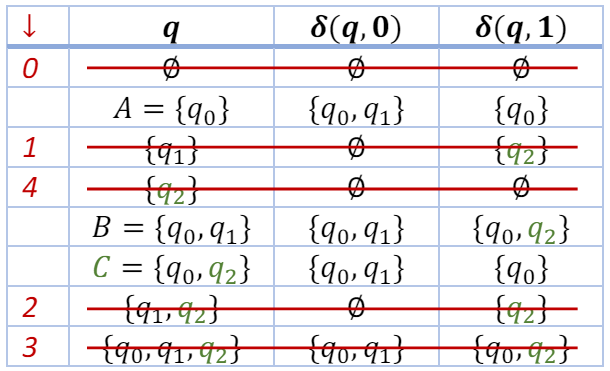
\includegraphics[width=1\linewidth]{images/teilmengenkonstruktion.png}
    \end{minipage}
    \begin{minipage}{0.5\linewidth}
        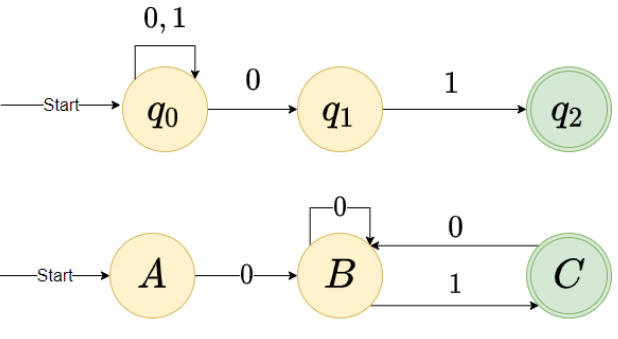
\includegraphics[width=1\linewidth]{images/teilmengenkonstruktion2.png}
    \end{minipage}
\end{formula}   

\begin{definition}{Zustandsklasse}
    $\Sigma^{*}=\bigcup_{p \in Q}[p] \quad [p] \cap[q]=\emptyset, \forall p \neq q, p, q \in Q$

    Jedes Wort landet in einem Zustand, aber kein Wort landet nach dem Lesen in zwei Zuständen!
\end{definition}

\begin{KR}{Zustandsklassen Beweis}
    Zeige: Jeder EA für die Sprache $L(M_9)=\{w \in\{0,1\}^{*} \mid| w|_{0} \bmod 3=1\}$ hat mindestens 3 Zustände.\\
    1. Jeder EA für $L\left(M_9\right)$ muss die Anzahl der gelesenen Nullen modulo 3 zählen und unterscheiden können.\\
    2. Zum Beispiel: $x_1=\varepsilon, x_2=0, x_3=00$\\
    3. Widerspruch für alle Paare von Wörtern aufzeigen:\\
    Für $x_1$ und $x_2: \quad z_{12}=\varepsilon \quad \Rightarrow \quad x_1 z_{12}=\varepsilon \notin L, \quad x_2 z_{12}=0 \in L$\\
    Für $x_1$ und $x_3: \quad z_{13}=0 \quad \Rightarrow \quad x_1 z_{13}=0 \in L, \quad x_3 z_{13}=000 \notin L$\\
    Für $x_2$ und $x_3: \quad z_{23}=\varepsilon \quad \Rightarrow \quad x_2 z_{23}=0 \in L, \quad x_3 z_{23}=00 \notin L$\\
    4. Jeder EA für $L\left(M_9\right)$ muss zwischen mindestens drei Zuständen unterscheiden. Der EA hat mind. 3 Zustände.
\end{KR}

\begin{example2}{NEA (nicht eindeutig)} Sprache: $L(M)=\left\{x 01 \mid x \in\{0,1\}^{*}\right\}$
    
    \begin{minipage}{0.5\linewidth}
        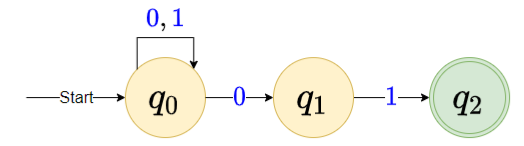
\includegraphics[width=1\linewidth]{images/nea_example1.png}
    \end{minipage}
    \hspace{1mm}
    \begin{minipage}{0.5\linewidth}
        \begin{center}
        \includegraphics[width=1\linewidth]{images/äquivalenter_nea.png}
        
        {\footnotesize äquivalenter DEA}
        \end{center}
    \end{minipage}    
\end{example2}



